\documentclass[11pt,a4paper,twoside]{book}
\usepackage[utf8]{inputenc}
\usepackage[italian]{babel}
\usepackage{amsmath}
\usepackage{amsfonts}
\usepackage{amssymb}
\usepackage[lmargin=3cm,rmargin=3cm,top=4cm,bottom=3cm]{geometry}
\usepackage{graphicx}
\usepackage{url}
\usepackage{listings} %Per inserire codice
\usepackage[usenames]{color} %Per permettere la colorazione dei caratteri
\usepackage[colorlinks=false]{hyperref}
\usepackage{verbatim}
\usepackage{pdfpages}
\addto\captionsitalian{%
\renewcommand{\lstlistingname}{Codice}}
\addto\captionsitalian{%
\renewcommand{\lstlistlistingname}{Elenco dei codici}}


\usepackage{pdfpages}
\author{Giulio Quarenghi}
\title{\large Specifica e diagnosi di sistemi attivi complessi}
\begin{document}
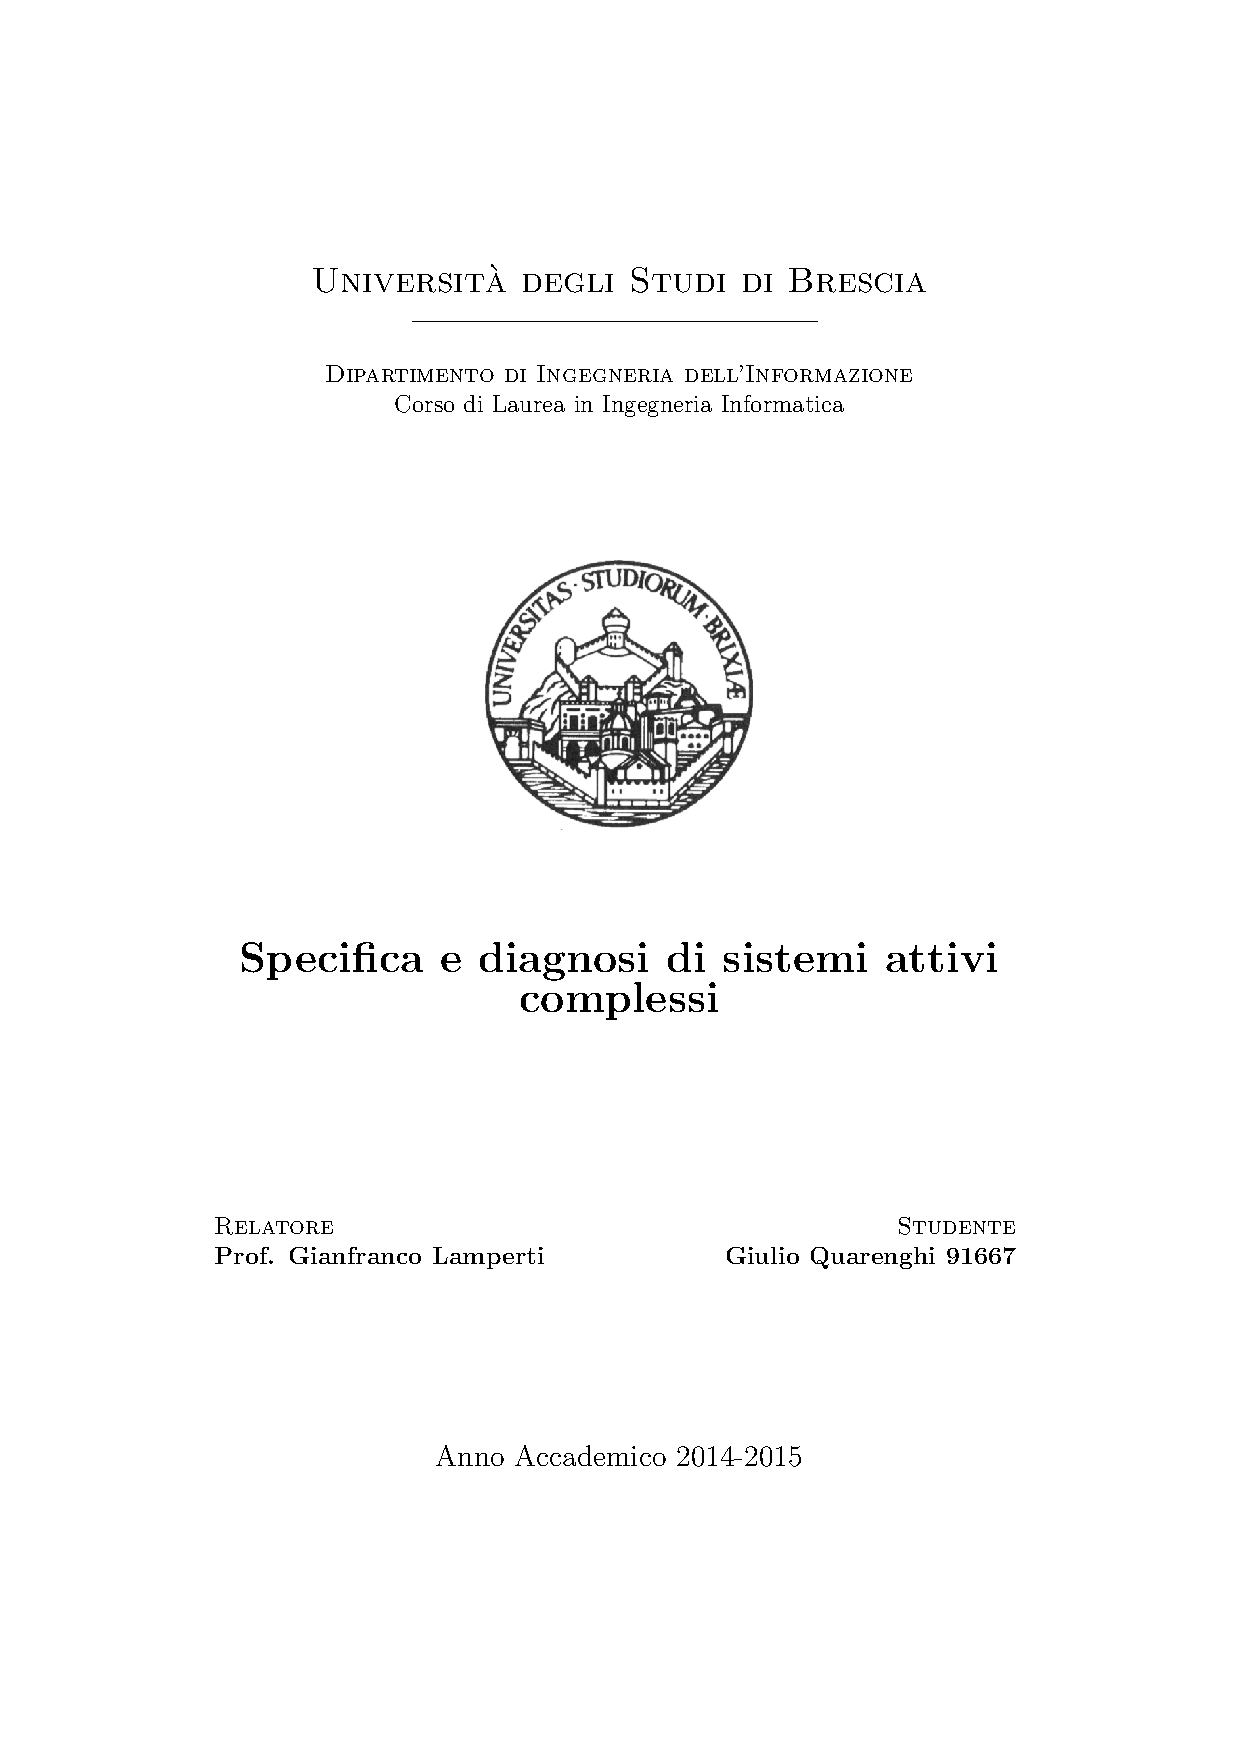
\includepdf[pages={1}]{frontespizio.pdf}
\frontmatter
	\tableofcontents
\mainmatter


\listoffigures

\nocite{*}
\bibliographystyle{unsrt}
\bibliography{bibliografia}
\addcontentsline{toc}{chapter}{\bibname}

\end{document}